The Self Organizing Map, SOM, introduced by Kohonen is a
non-supervised neural
learning algorithm. The map is composed of neighboring cells which are
in competition by means of mutual interactions and they adapt in order
to match characteristic patterns of the examples given during the
learning. The SOM is usually on a plane (2D).

The algorithm implements a nonlinear projection from a high
dimensional feature space to a lower dimension space, usually 2D. It
is able to find the correspondence between a set of structured data
and a network of much lower dimension while keeping the topological
relationships existing in the feature space. Thanks to this
topological organization, the final map presents clusters and their
relationships. 

%\subsection{The algorithm}
Kohonen's SOM is usually represented as an array of cells where each
cell is, $i$, associated to a feature (or weight) vector  $\underline m_i = \left[m_{i1},m_{i2},\cdots,m_{in}\right]^T\in
\mathbb{R}^n$ (figure \ref{carte}).\\
\begin{figure}
\center
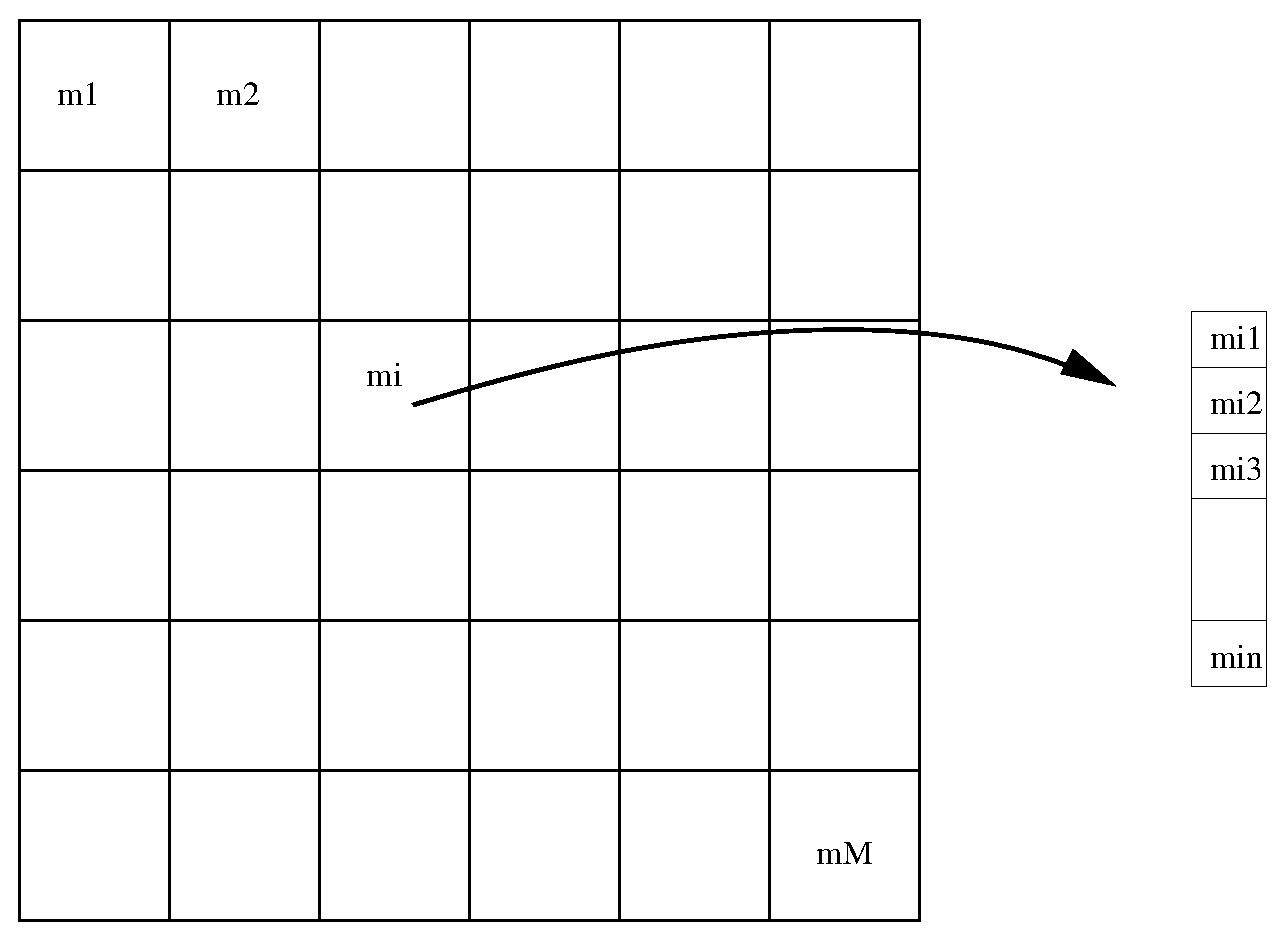
\includegraphics[width=0.45\textwidth]{carte.eps}
\itkcaption[Kohonen's Self Organizing Map]{Kohonen's Self Organizing Map}
\label{carte}
\end{figure}

A cell (or neuron) in the map is a good detector for a given input
vector $\underline x = \left[x_{1},x_{2},\cdots,x_{n}\right]^T\in
\mathbb{R}^n$ if the latter is {\em close} to the former. This
distance between vectors can be represented by the scalar product 
$\underline{x}^T\cdot\underline{m_i}$, but for most of the cases other
distances can be used, as for instance the Euclidean one. The cell
having the weight vector closest to the input vector is called the
{\em winner}.

%\subsubsection{Learning}
The goal of the learning step is to get a map which is representative
of an input example set. It is an iterative procedure which consists
in passing each input example to the map, testing the response of each
neuron and modifying the map to get it closer to the examples.

\begin{algo}
SOM learning:
\begin{enumerate}
\item $t=0$.
\item Initialize the weight vectors of the map (randomly, for instance).
\item While $t<$ number of iterations, do:
\begin{enumerate}
\item $k=0$.
\item While $k<$ number of examples, do:
\begin{enumerate}
\item Find the vector $\underline{m}_i(t)$ which minimizes the distance
$d(\underline{x}_k,\underline{m}_i(t))$
\item For a neighborhood $N_c(t)$ around the winner cell, apply the transformation:
\begin{equation}
\underline{m}_i(t+1)=\underline{m}_i(t)+\beta(t)\left[\underline{x}_k(t)-\underline{m}_i(t)\right]
\label{khoupdate}
\end{equation}
\item $k=k+1$
\end{enumerate}
\item $t=t+1$.
\end{enumerate}

\end{enumerate}
\end{algo}


In \ref{khoupdate}, $\beta(t)$ is a decreasing function with the
geometrical distance to the winner cell. For instance:
\begin{equation}
\beta(t)=\beta_0(t)e^{-\frac{\parallel \underline{r}_i -  \underline{r}_c\parallel^2}{\sigma^2(t)}},
\end{equation}
with $\beta_0(t)$ and $\sigma(t)$ decreasing functions with time and
$\underline{r}$ the cell coordinates in the output -- map -- space.\\

Therefore the algorithm consists in getting the map closer to the
learning set. The use of a neighborhood around the winner cell allows
the organization of the map into areas which specialize in the
recognition of different patterns. This neighborhood also ensures that
cells which are topologically close are also close in terms of the
distance defined in the feature space.

